\documentclass[fontsize=12pt,twoside=false,numbers=noenddot]{kaobook}

\usepackage{expex}
\usepackage{fontspec}
\usepackage{booktabs}
\usepackage{caption}
\usepackage{subcaption}
\usepackage[utf8]{inputenc}

%--- METADATA ---%
\newcommand{\langname}{\textbf{lang₂}}
\title[A Grammar of \langname{}]{\huge \langname{}}
\subtitle{grammar of a constructed language}
\author[kilenc]{\large Seth Thompson \\ \small \textit{aka} kilenc}
\date{\small \today}

%--- FORMATTING ---%
% font
\setmainfont{LibertinusSans}[Extension = .otf , Path = ./ , UprightFont = *-Regular-Custom , BoldFont = *-Bold-Custom , ItalicFont = *-Italic-Custom]
\setmonofont{Iosevka}[Scale=MatchLowercase]

% graphics
\graphicspath{{/}{images/}} % image paths

% links
\hypersetup{colorlinks=true, linkcolor=black, urlcolor=blue}

% romanization
\newcommand{\rzc}{\color[HTML]{5B2D90}}
\newcommand{\rz}[1]{\textit{\rzc #1}}

% foreign words
\newcommand{\fzc}{\color[HTML]{2D8F5B}}
\newcommand{\fz}[1]{\textit{\fzc #1}}

% proto words
\newcommand{\pzc}{\color[HTML]{8F5B2D}}
\newcommand{\pz}[1]{\textit{\pzc #1}}

% shortcuts for common stuff
\newcommand{\tsc}[1]{\textsc{#1}}
\newcommand{\tbs}{\textbackslash}
\newcommand{\ttd}{\char“~}
\newcommand{\tss}[1]{\textsuperscript{#1}}
\renewcommand{\bf}{\bfseries}
\renewcommand{\it}{\itshape}
\renewcommand{\sc}{\scshape}

% glossing style
\definelingstyle{gloss}{glstyle=nlevel, everyglpreamble=\bf\rzc, aboveglftskip=-8pt, belowglpreambleskip=-8pt, aboveexskip=0pt, belowexskip=-4pt}
\definelingstyle{widegloss}{glstyle=nlevel, everyglpreamble=\bf\rzc, aboveglftskip=0pt,belowglpreambleskip=0pt, aboveexskip=8pt, belowexskip=4pt}

\newenvironment{gloss}{
	\pex[lingstyle=gloss]%
}{%
	\xe%
}%

\newenvironment{gloss*}{
	\begin{minipage}{164.6mm}%
	\pex[lingstyle=widegloss]%
}{%
	\xe%
	\end{minipage}%
}%

\newcommand{\smoyd}[2]{\trailingcitation{\footnotesize \href{#1}{(\tsc{5moyd \#{}#2})}}}

\begin{document}

\frontmatter

% title page
\KOMAoptions{twoside=semi}
\maketitle
\KOMAoptions{twoside=false}

% toc
\setlength{\textheight}{23cm} % Manually adjust the height of the ToC pages
\etocstandarddisplaystyle % "toc display" as if etoc was not loaded
\etocstandardlines % toc lines as if etoc was not loaded
\tableofcontents 

% document start
\pagelayout{margin}

% introduction
\setchapterpreamble[u]{\margintoc}
\chapter{Introduction}
\section{Origins}
\langname{} is an \emph{a priori} artlang originally conceived to fulfill a speedlang challenge, then modified to handle a relay, then finally molded into its own project. Although I had no clear motivations in mind when beginning it, I found that the confluence of random decisions---the Gleb-generated inventory, challenge stipulations, the early translation choices---made the project into something I really enjoyed.

\section{Goals}
The overarching goal is to create something that is cool to me. The project is meant to be naturalistic, but when naturalism conflicts with aesthetic, aesthetic will be prioritized.

A primary way to grow this language and develop new ideas will be through translation of poetry and scientific journals. I hope that these will push the limits of my syntactical rules while also developing an interesting corpus. I'll also try to use \tsc{5moyd}s and hopefully at some point a journal to expand my ability to speak the language and get an intuitive sense for what constructions it prefers.

As I develop this conlang, my goals will be to explore analytic constructions and syntactic minutiae, write in-depth documentation of how information structure manifests in the language, and produce a robust dictionary and corpus.

\section{Lore}
\langname{} is set in a worldbuilding project I create as a hobby. The language is an isolate spoken on the eastern coast of a peninsula, once the language of city-states and now a common language throughout a number of coastal countries. It is heavily influenced by East Cape, the \emph{de jure} language of the peninsula, and other languages of trade. The world the speakers know is analogous to our 1930s.

\mainmatter

\pagelayout{wide} \part{Phonology} \pagelayout{margin}

\setchapterpreamble[u]{\margintoc}
\chapter{Segments}
\section{Consonants}
\langname{} has 14 consonant phonemes, although some newer analyses also analyze voiced stops as phonemic as wells. There are four distinguished places of articulation: labial, plain alveolar, sibilant alveolar, \marginnote[*-2]{The \emph{sibilant} place of articulation is a sprachbund feature, present in other Peninsular languages including East Cape.} and dorsal. There are four distinguisheds manner of articulation: stops, fricatives, approximants, and nasals.

\begin{table}[h] \centering
    \begin{tabular}{c|cccccccc}
        \toprule
        & \multicolumn{2}{c}{\bf Labial} & \multicolumn{2}{c}{\bf Alveolar} & \multicolumn{2}{c}{\bf Sibilant} & \multicolumn{2}{c}{\bf Dorsal} \\
        \midrule
        \bf{Stop}           & p & \it\rzc p & t & \it\rzc t & t͡s & \it\rzc c & k & \it\rzc k \\
                            & (b) & \it\rzc b & (d) & \it\rzc d & (d͡z) & \it\rzc j & (g) & \it\rzc g \\
        \bf{Fricative}      & f & \it\rzc f & ɬ & \it\rzc l & s & \it\rzc s & x & \it\rzc h \\
        \bf{Nasal}          & m & \it\rzc m & n & \it\rzc n & n͡z & \it\rzc z \\
        \bf{Approximant}    & w & \it\rzc v & ɹ & \it\rzc r & & & j & \it\rzc y \\
        \bottomrule
    \end{tabular}
    \caption{Consonants}
    \end{table}

\paragraph{Nasal Sibilant}
The nasal sibilant /n͡z/ is a typologically odd segment. The prototypical representation of this sound is [z̃], a voiced fricative with simultaneous nasal release; however, phonetic research\marginnote{See \href{https://www.icacommission.org/Proceedings/ICA1998Seattle/pdfs/vol_4/2921_1.pdf}{Ohala et al. (1998)} for further discussion of nasal fricatives.} suggests that true fricatives cannot be fully nasalized. Thus, this segment's typical realization may be better represented as a slightly fricated approximant [\tss{n}z̞̃], although some speakers may realize it as a weakly nasalized [\tss{n}z] or a fully nasalized approximant [\tss{n}ɹ̃]. Nevertheless it patterns as a nasal sibilant in both distribution and allophony and is thus phonemically represented as /n͡z/.

\paragraph{Labial Fricative}
The fricative /f/ has a marginal distribution, mostly appearing in loan words and onomatopoeia. Most instances of historical /f/ underwent debuccalization and were subsequently lost. Although /x/ also appears frequently in onomatopoeia, its distribution is more widespread and it is not considered marginal.

\paragraph{Sibilant Affricate}
Although the phone [t͡s] is rather common in the corpus, its underlying form is not always the phoneme /t͡s/. \marginnote{Affrication of stop-fricative clusters and pre-[s] schwa deletion are common processes that yield [t͡s], discussed further in §\ref{sec:conso_morphono}.} The underlying phoneme is usually elucidated by inflection. For example, both \rz{tsekla} “steering wheel” and \rz{cekla} “great uncle” share the same surface form, [ˈt͡sekɬə]. However, when inflected for the plural, the former becomes [ˌtasəkˈɬaz̃əɹ] and the latter [t͡səkˈɬaz̃əɹ]. As such \rz{tsekla} is analyzed as /tasekɬa/, whereas \rz{cekla} is analyzed as /t͡sekɬa/. This analysis parallels liason in some languages.

\section{Vowels}
\langname{} has 8 vowel phonemes, 5 plain and 3 nasalized. 

\begin{table}[h] \centering
\begin{tabular}{c|cccccccccccc}
    \toprule
    & \multicolumn{4}{c}{\bf Front} & \multicolumn{4}{c}{\bf Mid} & \multicolumn{4}{c}{\bf Back} \\
    \midrule
    \bf High & i & \it\rzc i & & & & & & & u & \it\rzc u \\
    \bf Mid & e & \it\rzc e & ẽ & \it\rzc ę & (ə) & \it\rzc a & (ə̃) & \it\rzc ą & o & \it\rzc o & õ & \it\rzc ǫ \\
    \bf Low & & & & & a & \it\rzc a & ã & \it\rzc ą \\
    \bottomrule
\end{tabular} 
\caption{Vowels}
\end{table}

\begin{kaobox}[frametitle=\sc todo:]
This section about vowel neutralization probably belongs in morphophonology? It also has to do with the supersegment stress.
\end{kaobox}

\paragraph{Vowel Neutralization} 
Mid and low vowels /e a o/ and their nasal counterparts are reduced to [ə ə̃] in unstressed syllables. \marginnote[*-2]{The surface form is typically romanized \rz{a} even for underlying /e o/. Dictionaries typically denote the \emph{shadow vowels} as \rz{nbm.}, an abbreviation of \rz{nabam} “shadow.”} Schwa is not phonemic, but neutralization is common, so it appears frequently throughout the corpus. In speech, the underlying vowel becomes evident when stress is shifted due to morphological processes.

\section{Allophony}

\setchapterpreamble[u]{\margintoc}
\chapter{Supersegments}
\section{Stress}
Stress in \langname{} is lexically and morphologically productive. Stress typically falls on the penultimate syllable of a word. Atypical vowel stress, most common in loan words, is marked with an acute. \marginnote{For example, \rz{tąka} “tree” has typical stress and is unmarked, but \rz{tąká} “reindeer” has atypical ultimate stress and is thus marked.} Stress is also morphologically productive, distinguishing between unmarked and distal deixis in nouns. Affixation, compounding, and other stress-shifting processes often cause stress-based minimal pairs to become homophones.

Stressed vowels have three phonetic differences from unstressed vowels. First, they typically have a rising pitch. Second, they are typically longer than unstressed vowels. Third, onsets before long vowels have a longer VOT than other onsets, a manifestation of slight aspiration or breathiness.

Secondary stress falls on alternating syllables starting from primary stress and spreading left. For example, \rz{kagęsa} “army” has regular stress on the penultimate syllable, but when inflected in plural form, it surfaces as \rz{kegąsazar} [ˌke.gə̃ˈsa.z̃əɹ]. Secondary stress prevents the reduction of /e a o/ to [ə], but, unlike primary stress, does not cause length or VOT increase.

\setchapterpreamble[u]{\margintoc}
\chapter{Morphophonology}
\begin{kaobox}[frametitle=\sc todo:]
This all just got recently moved from allophony because it's better analyzed as a morphophonological phenomenon, probably. So some of it will have to be re-written with that framing in mind. Probably means a lot more double slashes and “it only occurs across morpheme boundaries” type stuff.
\end{kaobox}
\section{Consonants} \label{sec:conso_morphono}
\paragraph{Voicing}
Nasal and stop clusters are realized as voiced stops, occasionally prenasalized. The resulting phones [\tss{(m)}b \tss{(n)}d \tss{(n)}d͡z \tss{(ŋ)}g] are romanized \rz{b d j g}. \marginnote{These clusters assimilate in place to the stop, so /np/ surfaces as [b], not as [d].} Clusters where the nasal is the onset of a syllable, not a coda, do not assimilate, so /pn/ is still realized [pn]. 

Although the assimilation process is most common across morpheme boundaries or in loan words, voiced plosives can be found in some native morphemes. However, since these phones only occur word-medially in limited and predictable distribution, they are not tradtionally considered phonemic. \marginnote{Some scholars argue that voiced plosives are phonemic or becoming phonemic because of their presence in loan words and verb conjugations.} Most native words with voiced plosives are transparent compounds, such as \rz{ebar} “below” (← \rz{ez} + \rz{par}) or \rz{kagęsa} “army” (← reduplication of \rz{kęsa}).

Some words, especially some conjugations of \rz{m}-stem verbs, are spelled with a word-final voiced stop, but the stop is still typically realized as a medial cluster. For example, \rz{sed} “they tell me” is underlying /semt/ and realized [se\tss{(n)}d(ə)]. For some speakers, especially younger speakers or those in informal contexts, the final schwa is elided.

\begin{kaobox}[frametitle=\sc todo:]
Affrication and assibiliation would make more sense if it was only accross morpheme boundaries, but I have some words that I like where it's morpheme-internal. How should I handle that? It could be reworked as a diachronic process, made phonemic, a morphophonemic process---but it needs more thought.
\end{kaobox}

\paragraph{Affrication}
Alveolar plosive and fricative clusters are realized as a sibilant affricate. Clusters of /ts/, /tf/, /tɬ/ and /tx/ all neutralize to [t͡s], romanized as \rz{c}. The /tn͡z/ cluster likewise affricates, but is realized as [t͡s̞̃], romanized as \rz{cz}. \marginnote[*-2]{The voiceless nasal affricate is notoriously hard for non-native speakers to pronounce and is often used as a shibboleth.}

\paragraph{Assibilation}
Sibilant and non-sibilant fricative clusters are realized as sibilants. Unvoiced sibilants /t͡s s/ clustering with /f x ɬ/ are realized as [sː], romanized as \rz{cc} or \rz{ss} depending on the underlying phoneme. The voiced sibilant /n͡z/ instead is realized as [z̞̃ː] in such clusters, romanized as \rz{zz}.

\section{Vowels}
\paragraph{Schwa Deletion}
The reduced vowel [ə] is often deleted between consonants,\marginnote{Nasalized schwa [ə̃] rarely undergoes deletion as it is typically longer than [ə].} especially non-alveolar stops, and the sibilants /t͡s s n͡z/. For example, \rz{ksarat} /kosaɹat/ is commonly realized as [ksaɹət], and spelled accordingly. The elision process results in word-final or word-initial [s]\marginnote{Note that /t͡s/ surfaces [s] in these environments.} or [z̃] being the only syllable-internal clusters. However, these clusters are not consistently realized, and occasionally have an epenthetic schwa, especially word-finally. 

\begin{kaobox}[frametitle=\sc todo:] 
Something here about word-final clusters. I haven't been consistent about when it's spelled as a cluster or when it's spelled with the vowel, and I need to either commit to the inconsistency, or figure out how that works.
\end{kaobox}

\begin{kaobox}[frametitle=\sc todo:] 
There might end up being an isogloss map of schwa deletion: most dialects delete ahead of sibilants, some ahead of sibilants and approximants, and others in all environments?
\end{kaobox}

\setchapterpreamble[u]{\margintoc}
\chapter{Phonotactics}
\section{Roots}
\paragraph{Nouns}
Most nominal roots are of the form CV(C)CV. Nominal roots infrequently end in a consonant, typically /s/ or /r/ for neuter nouns. Rarely, nominal roots end in /m n/ or /k/.

\paragraph{Verbs}
Most verbal roots are of the form (C)VC or CV(C)CVC. /t/ is the most common root-final phoneme, although there are some /m/ and /r/ stems as well.

\paragraph{Affixes}
A smaller set of phonemic segments are allowed in affixes. Neither the labials /p f m w/ nor the high vowel /u/ appear in true affixes.\marginnote{Because /u/ and /w/ pattern similarly, some phonemic analyses conflate them.} In the fossilized partial reduplication process, the reflexes of labial are either /k/ (← /p f/) or /n/ (← /m w/). The high vowel /u/ lowers to /o/, often simply realized as [ə].

\section{Frequencies}
\begin{kaobox}[frametitle=WIP Lexifer file]
\begin{verbatim}
with: std-ipa-features coronal-metathesis

letters: a ą b c d e ę f g h i k l m n o ǫ p r s t u v y z 

C = t s k n y h r c m z l p v f
N = s r m n k
P = t m r
V = a e i ą o ę ǫ u

random-rate: 40
words:  CVC?CVN? C?VC?CVP C?VP C?VN?

filter: mt > d; nt > d; zt > d; mc > j; nc > j; zc > j; mk > g; nk > g; zk > g; mp > b; np > b; zp > b; ts > c; tl > c; th > c; tf > c; tz > cz; sc > ss; sl > ss; sh > ss; sf > ss; cs > cc; cl > cc; ch > cc; cf > cc; zs > zz; zc > zz; zf > zz; zl > zz; zh > zz;
\end{verbatim}
\end{kaobox}

\pagelayout{wide} \part{Morphosyntax} \pagelayout{margin}

\setchapterpreamble[u]{\margintoc}
\chapter{Nouns}
The \langname{} noun phrase is largely analytic, but nouns do inflect for deixis and number. % Nouns have three broad inflection patterns, largely related to the way they inflect for plurality.

% \section{Stems}
% Nouns are broadly divided into three stems based on their inflectional patterns: \emph{vocalic}, \emph{\rz{s}-stems}, and \emph{\rz{r}-stems}. Rarely noun stems will end in other consonants, but these have no discernible shared patterns and often comprise newer loans.

% Most noun stems are vocalic stems; typically these end in mid vowels, although some do end in a high vowel. Vocalic stems are usually common gender, excluding loanwords, which are prescriptively assigned neuter gender even if they end in a vowel. 

% Neuter nouns, on the other hand, are often either \rz{r}-stems or \rz{s}-stems, the latter being more common. \marginnote{\rz{S}-stems can end in any sibilant, typically \rz{-s} but also \rz{-c} or \rz{-z}.} Although no longer morphologically productive, the endings on \rz{s}-stems and \rz{r}-stems derive from historical derivation processes. Many roots are reflected in both endings, but the shared meaning between them is not always transparent.

% \subsection{Vocalic stems}
% Vocalic stems have fairly regular, agglunative inflection patterns. However, the proximal plural is shortened to \rz{-rran} for most speakers.

% \begin{table}[h] \centering
%     \begin{tabular}{c|ccc}
%         \toprule
%         & \bf Generic & \bf Proximal & \bf Distal \\
%         \midrule
%         \bf \sc sg & \it\rzc metka & \it\rzc metkan & \it\rzc matkó \\
%         \bf \sc pl & \it\rzc matkozar & \it\rzc matkorran & \it\rzc matkazár \\
%         \bottomrule
%     \end{tabular}
%     \caption{Inflection of vowel-stem \rz{metka} “bowl”}
%     \label{tab:metka_inflection}
% \end{table}

% All vocalic forms share the same endings, but many will have an unpredictable final vowel due to stress-based mid vowel neutralization. There is no way to predict the final vowel from the uninflected lemma, so learners often resort to memorization.

% \subsection{Neuter stems}
% Neuter stems share a common inflection pattern. For both neuter stems, the proximal surfaces as /on/ instead of /n/. The proximal plural also shortens for neuter stems, but takes the form \rz{-zza-}, influenced by the assibilation morphophonological process. The shared plural form for both stems can create homophones.\marginnote[*-2]{Some strategies to resolve homophones are covered in §\ref{subsec:additive_plural}.} 

% \begin{table}[h] \centering
%     \begin{tabular}{c|ccc}
%         \toprule
%         & \bf Generic & \bf Proximal & \bf Distal \\
%         \midrule
%         \bf \sc sg & \it\rzc retus & \it\rzc ratusan & \it\rzc ratús \\
%         \bf \sc pl & \it\rzc ratuzzar & \it\rzc ratuzzan & \it\rzc ratuzzár \\
%         \bottomrule
%     \end{tabular}
%     \caption{Inflection of \rz{s}-stem \rz{retus} “blade”}
% \end{table}

% \begin{table}[h] \centering
%     \begin{tabular}{c|ccc}
%         \toprule
%         & \bf Generic & \bf Proximal & \bf Distal \\
%         \midrule
%         \bf \sc sg & \it\rzc pebar & \it\rzc pabaran & \it\rzc pabár \\
%         \bf \sc pl & \it\rzc pabazzar & \it\rzc pabazzan & \it\rzc pabazzár \\
%         \bottomrule
%     \end{tabular}
%     \caption{Inflection of \rz{r}-stem \rz{pebar} “garden”}
% \end{table}

\section{Deixis}
Nominal deixis has a variety of uses, including evidentiality, distance, familiarity, and topicality.\marginnote{I had this idea, then found out that, as usual, a natural language had it first. Read \href{http://lingpapers.sites.olt.ubc.ca/files/2020/07/11_ICSNL55_Huijsmans_Reisinger_Matthewson_final.pdf}{Huijsmans, Reisinger, and Matthewson (2020)} for more about the Salishan languages.} Verbs and adjectives exhibit agreement for deictic reference. There are three deictic categories: \emph{generic}, \emph{proximal}, and \emph{distal}.

Although diachronically related to demonstratives, spacial deixis is only a secondary use of the proximal and distal forms. Instead, they are primarily indicators of non-propositional evidentiality, \tit{i.e.} the speaker's evidence of a nominal referent. Evidence in this sense is visual or non-visual, the latter largely encoding hearsay or inference. The non-propositional evidentiality system in \langname{} is semantically based on the speaker's knowledge at or prior to speech time.\marginnote{\href{https://ditibhadra.com/chapter_draft.pdf}{Bhadra (2020)} terms this a Type I system.} 

\subsection{Generic}
The generic form of the noun is morphologically least marked and used as the citation form.

The generic form is most often used for gnomic statements.

\begin{gloss}
    \begingl
        \glpreamble Kęsa esyi oc. \endpreamble
            kęsa[hero]
            esyi[good]
            ot-s[be-\tsc{3c}]
        \glft “Heroes are good.”
    \endgl
\end{gloss}

The referent \rz{kęsa} is unmarked to convey that the speaker means heroes in the general sense, not a specific person. Compare (\lastx) with (\nextx), which both refer to a specific hero.

\begin{gloss}
    \a \begingl
        \glpreamble Kęsan esyin ací. \endpreamble
            kęsa-n[hero-\tsc{prox}]
            esyi-n[good-\tsc{prox}]
            ot-s-í[be-\tsc{3c-prox}]
        \glft “The hero (I know) is good.”
    \endgl
    \a \begingl
            \glpreamble Kąsá asyí aséc. \endpreamble
                kęsa[hero\tbs\tsc{dist}]
                esyi[good\tbs\tsc{dist}]
                ot-s[be-\tsc{3c}\tbs\tsc{dist}]
            \glft “The hero (I've heard of) is good.”
    \endgl
\end{gloss}

If direct or indirect evidence exists, it's infelicitious to use the generic form.

\subsection{Proximal}
The proximal form of a noun is used when the speaker is certain, nearby, or familiar with the noun.
%It can also be used for the conversational topic.
This form most commonly denotes direct evidence, meaning the speaker has personal experience with the marked noun. It is marked with the suffix \rz{-n}. \marginnote[*-2]{\rz{-n} is morphophonemically ⫽on⫽, where ⫽o⫽ doesn't surface for vocalic stems.}

\paragraph{Direct evidence}
The canonical meaning of the proximal form is direct evidence, often translated as “I saw.” 

\begin{kaobox}[frametitle=\sc todo:]
    The definiteness constructions probably need to be reworked to square better with (a) the stuff I've learned about definiteness and (b) the use of the deictic forms for topic/focus.
\end{kaobox}

\paragraph{Definiteness}
Proximal forms can be used to describe the definiteness of a referent. This construction is only used for weak, uniqueness-based definiteness (eg. “the Moon”), never for strong, anaphoric definiteness (eg. “the book”). For strong definitess, the noun \rz{sin} “???” is used alongside distal form, as in (\nextx b).

\begin{gloss*}
    \a \begingl
        \glpreamble Nassoin kąstecik su kagęsa su kagę́stapa. \endpreamble
            nassoi-n[king-\tsc{prox}]
            kąstecik[command]
            su[and]
            kagęsa[army]
            su[and]
            kagę́stapa[navy]
        \glft “The king (that we know) commands both army and navy.”
    \endgl
    \a \begingl
        \glpreamble sah ez-Rosąm pít ató sín. \endpreamble
            sah[soon]
            tę=rosąm[\tsc{prep}=cook]
            pít[hold\tbs\tsc{dist}]
            ató[grain\tbs\tsc{dist}]
            sín[???\tbs\tsc{dist}]
        \glft “The rice (that you mentioned) is about to be cooked.”
        \smoyd{https://www.reddit.com/r/conlangs/comments/kck1hi/1381st_just_used_5_minutes_of_your_day/}{1381}
    \endgl
\end{gloss*}

\subsection{Distal}
The distal form of a noun is used when the speaker is uncertain, far, or unfamiliar with the noun. 
%It can also be used for the conversational focus.
This form typically denotes indirect evidence, including inference, meaning the speaker has heard of or can make an educated guess about the existence of the marked noun. Reported deixis is marked by shifting stress to the ultimate syllable of the word.

\paragraph{Indirect Evidence}
The prototypical meaning of the distal form is indirect evidence, often translated as “heard about” or “they said.” As in (\nextx), this evidence is encoded into the clause via the subject and the predicate that agrees with it.

\begin{example*}
    \script egi Matkó aczé samséc lar tę-het.
    \bits egi matkó aczé samséc lar tę=het
    \gloss just basket\tbs\tsc{dist} two\tbs\tsc{dist} will:be\tbs\tsc{dist} there to=be:at
    \tr (She said) there will be just two baskets.
    \smoyd https://www.reddit.com/r/conlangs/comments/ic7on8/1314th_just_used_5_minutes_of_your_day/ & 1314
\end{example*}

\section{Number}
Nouns inflect morphologically for an additive plural, but there is also a syntactic construction used to form associative plurals. The unmarked form of a noun encodes expected number, \eg \rz{parsa} “eyes” which defaults to a pair and must be modified by a numeral or appositive to specify a singulative. 

\begin{figure}[h]
    \centering
    \begin{subfigure}{0.4\textwidth}
        \centering
        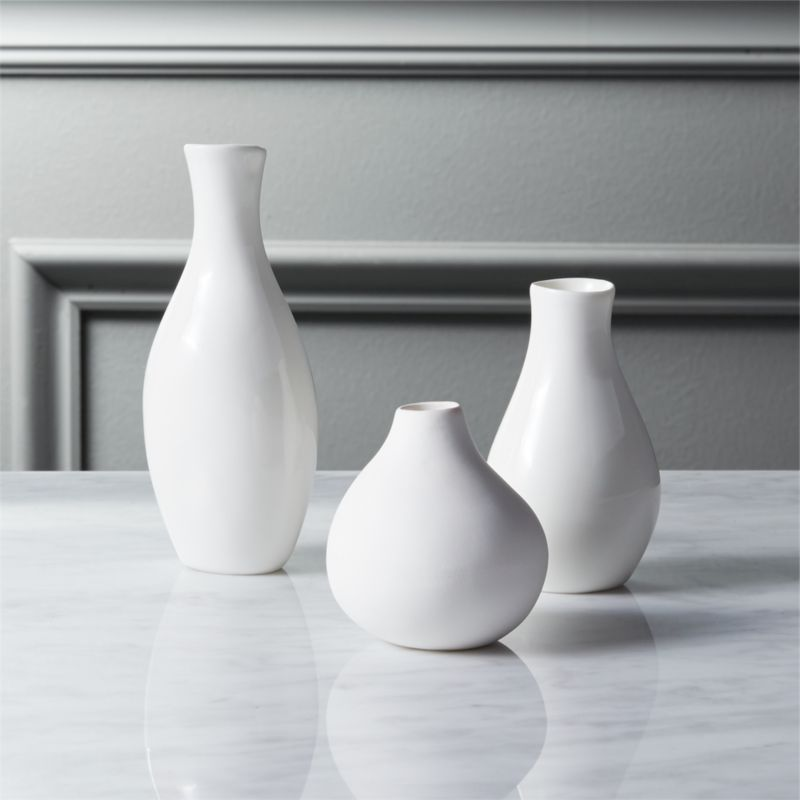
\includegraphics[width=\textwidth]{same_vases.jpg}
        \caption{\rz{matkozar}}
    \end{subfigure}
    \begin{subfigure}{0.4\textwidth}
        \centering
        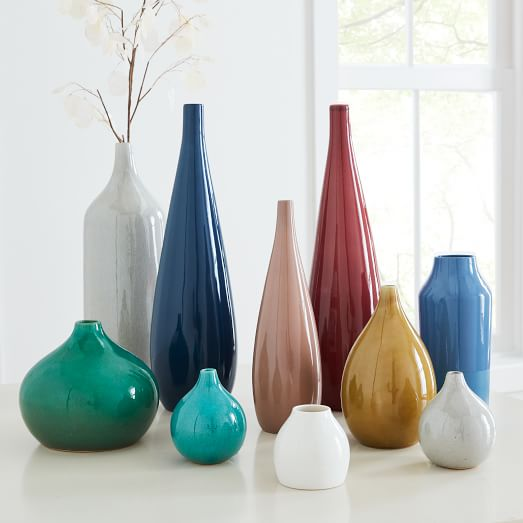
\includegraphics[width=\textwidth]{different_vases.jpg}
        \caption{\rz{ezzu metka}}
    \end{subfigure}
    \caption{Additive vs. associative plurals}
\end{figure}

The primary difference in the two plurals is the composition of the set: additive plurals refer to largely homogenous referents, whereas associative plurals refer to largely heterogenous referents.

\subsection{Additive plurals} \label{subsec:additive_plural}
Additive plurals are used for a set of homogenous referents and never heterogenous referents; \eg \rz{matkozar} is “a set of the same (or similar) bowl” and never “a set of diverse bowls.”\marginnote{The second meaning would use the associative plural.}

Additive plurality is indicated through the suffix \rz{-zar}. Morphological marking is optional and a noun can be inferred additively plural from context. \marginnote{Mandatory plural marking is stylistically preferred in formal contexts.} As such marking is less common for small, discrete or easily countable sets or when a referent has been established plural in prior conversation. However, speakers are not always consistent with marking.

Morphonologically, plural marking can be thought to precede deictic marking; plural distal nouns have accent placed on the plural suffix. As seen in Table \ref{tab:metka_inflection}, \rz{matkozar} becomes \rz{matkazár}, not \rz{*matkózar}.

\paragraph{Combating homophony}
Because the suffixes of \rz{s}-stems and \rz{r}-stems merge in the plural, some minimal pairs are rendered homphones when inflected. To combat this, speakers sometimes employ \rz{tevi} “many” as an appositive modifier for the singular form.

\paragraph{Explicit number}
When number is specified with a numeral, the noun is not marked for plurality, as in (\nextx). This can also be used as another strategy to combat homophony.

% \begin{gloss}
%     \begingl
%         \glpreamble vęci ocza \endpreamble
%             vęci[mercenary]
%             ocza[two]
%         \glft “two mercenaries”
%         \trailingcitation (cf. \rz{vącizar} “mercenaries”)
%     \endgl
% \end{gloss}

\subsection{Associative plurals}
Unlike the additive plural, the associative plural is not marked morphologically; it is nonetheless rather prevalent. The preposition \rz{ezzu} conveys the associative meaning.\marginnote{Like \rz{su}, \rz{ezzu} can appear stranded. See §\ref{subsec:u_and_su}.}

The associative is used for a set of heterogenous referents. For animate (especially human) referents, the meaning is canonically “a person and their associates,” as in (\nextx). The focal referent\marginnote{Terminology in this section adapted from \href{https://amor.cms.hu-berlin.de/~h2816i3x/Lehre/2007_VL_Typologie/03_Daniel_AssociativePlural.pdf}{Daniel and Moravcsik (2007)}.} (\ie most important) is the marked noun.

% \begin{gloss}
%     \begingl
%         \glpreamble Sayanarnat otik ezzu Kanyi ez-laran. \endpreamble
%             sayenar-nat[be.ignorant-\tsc{cvb}]
%             ot-ik[be-\tsc{prox}]
%             ezzu[\tsc{assoc}]
%             Kanyi[\tsc{name}]
%             ez=lar-n[\tsc{prep=expl-prox}]
%         \glft “For this, Kanyi and his friends won't be much \emph{help}.”
%     \endgl
% \end{gloss}

However, the associative can also have a number of idiomatic, context-specific meanings, usually referring to diverse groups.

% \pex 
% \a \begingl
% \glpreamble ezzu Akakvazi rematt \endpreamble
% \glft “The diverse group of tag players entertained us ...”
% \endgl 
% % \a \begingl
% % \glft “My grandfather painted a wide variety of paintings.”
% % \endgl
% \xe

\section{Gender}
Although nouns traditionally distinguish \emph{common} and \emph{neuter} gender, this has largely become a prescriptive convention. \marginnote{The gender distinction is more common in literature or academia.} Loanwords, especially technical loanwords, are typically assigned neuter gender. Some words only distinguish gender for certain uses or contexts, thus dictionaries typically denote if a given usage is expected to require neuter gender.

\section{Apposition}
Apposition is fairly common due to the small adjective class present in \langname{}. Apposition is used in a number of collocative constructions but is distinct from compounding largely because of stress patterns and morphophonological processes.\marginnote{Compounds can shift stress and also show cross-morpheme sound changes.} Furthermore, appositive nouns shown agreement with the noun they modify, like adjectives.

\subsection{Inalienable possession}
Apposition is a fairly common strategy for possession of all types,\marginnote{Alienable possession via apposition is dispreferred in formal registers.} but inalienably possessed nouns require apposition, as in (\nextx b).

% \begin{gloss}
%     \a \ljudge{?} \begingl 
%         \glpreamble  hora im-kęsa \endpreamble
%         hora[wrist]
%         im=kęsa[of=soldier]
%         \glft \textit{Intended:} “soldier's wrist”
%     \endgl
%     \a \begingl 
%         \glpreamble hora kęsa \endpreamble
%         hora[wrist]
%         kęsa[soldier]
%         \glft “soldier's wrist”
%     \endgl
% \end{gloss}

The sentence in (\lastx a) more readily lends itself to a reading indicating inalienable possession, such as “soldier's craftmanship” or “soldier's weaponsmithing.”

\subsection{Reducing syntactic complexity}
Appositives are also used as a way of combating heaviness in complex noun phrases. This often occurs in noun phrases with multiple prepositional modifiers, especially when one of the modifiers is \rz{im} “of.” Other prepositions can be reduced this way as well. 

When multiple prepositional phrases modify a head noun the phrase is syntactically heavy. For example (\nextx) has three modifiers, an adjective and two prepositional phrases, one with its own adjective.

% \begin{gloss*}
%     \begingl
%         \glpreamble rat Hecik pakné taá im-lalasan ez-helazzaran acoan. \endpreamble
%         rat[I]
%         hecik[be.at]
%         pakné[house\tbs\tsc{dist}]
%         taá[blue\tbs\tsc{dist}]
%         im=lalasa-n[of=auntie-\tsc{prox}]
%         ez=helazzaran[\tsc{prep}=mountains]
%         acoan[tall]
%         \glft “I'll be at auntie's blue house near the tall mountains.”
%     \endgl
% \end{gloss*}

To reduce the syntactic load of the sentence, a speaker might instead render it as (\nextx). The phrase is clearly appositional; \rz{lalasa} switches from proximal marking (indicating the speaker has met her) to distal marking (to agree with its head noun). 

% \begin{gloss*}
%     \begingl
%         \glpreamble rat Hecik pakné taá lalasá ez-helazzaran acoan. \endpreamble
%         rat[I]
%         hecik[be.at]
%         pakné[house\tbs\tsc{dist}]
%         taá[blue\tbs\tsc{dist}]
%         lalasá[auntie\tbs\tsc{dist}]
%         ez=helazzaran[\tsc{prep}=mountains]
%         acoan[tall]
%         \glft “I'll be at auntie's blue house near the tall mountains.”
%     \endgl
\end{gloss*}

The new sentence has fewer function words and less disparate inflections, reducing some of its complexity.

\section{Phrasal syntax}
Noun phrases are predominantly head-initial. Generally speaking, syntactically simpler consituents occur before more syntactically complex ones, as shown in (\nextx).

\begin{example}
    head → adjective → number → appositive → prepositional phrase
\end{example}

\setchapterpreamble[u]{\margintoc}
\chapter{Pronouns}
Prounouns are morphologically and syntactically similar to other nouns---they share inflectional patterns and can be modified by adjectives. The notable differences are that pronouns rarely inflect for deixis, and some appositive constructions are ungrammatical.

\begin{kaobox}[frametitle=\sc todo:]
Settle on pronominal forms---right now it's \rz{rat} \tsc{1}, \rz{a(f)} \tsc{2}, \rz{sec} \tsc{3c}, and \rz{moc} \tsc{3n}. There's some isogloss map about whether \tsc{2} is \rz{a} or \rz{af}.
\end{kaobox}

\paragraph{Possession}
Like nominal possession, pronominal possession can be expressed either through apposition or prepositional phrases. \marginnote{Formal registers prefer the prepositional construction.} Thus both \rz{lar im-sec} and \rz{lar sec} can mean “his thing.” However, apposition is more common in isolation for pronouns than it is for nouns.

\setchapterpreamble[u]{\margintoc}
\chapter{Verbs}
Like the noun phrase, the \langname{} verb phrase is mostly analytic, and inflection is largely reserved for agreement. Other parts of the verb complex are handled by periphrastic constructions, notably including valency operations and TAM.

\section{Agreement}
Verbs display agreement along two axes: \emph{deixis} and \emph{person}. Deictic agreement is only with the subject of the clause, but person agreement\marginnote[*-1]{Despite person agreement, \langname{} is rarely pro-drop.} is with both subject and the object, if the verb is transitive. Only the sole finite verb of a clause bears agreement; verbs demoted to adjuncts or arguments are always uninflected.

\subsection{Person}
In old \langname{}, verb agreement was transparently derived from cliticized pronouns. However, sound change reduced agreement endings, leading to synchronic forms that are often actually patient agreement.

\begin{kaobox}[frametitle=\sc todo:]
	How to cover morphophonological stuff? The two main ones are affrication of /t/ + /s z/ and cluster-final /s ts/ merging to [s], spelled \rz{s}.
\end{kaobox}

\begin{margintable} \centering
	\begin{tabular}{cc}
		\toprule
		\bf Morpheme & \bf Meaning \\
		\midrule
		\it -\rz{rc}- & \sc 1.ag \\
		\it -\rz{r}- & \sc 1.pt \\
		\it -\rz{a}- & \sc 2 \\
		\it -\rz{s}- & \sc 3c \\
		\it -\rz{z}- & \sc 3n \\
		\it -\rz{ns}- & \tsc{1}↔\tsc{3n} \\
		\it -\rz{k}- & \sc refl \\
		\bottomrule
	\end{tabular}
	\caption{Summary of person agreement}
	\label{tbl:person}
\end{margintable}

Except in a few outlier cases, agreement is fairly predictable from Table \ref{tbl:person}. Neuter agreement takes precedent over other morphemes when applicable. Furthermore, -\rz{a}- only appears on intransitive verbs; for transitive verbs, the appropriate agreement with the other argument is used instead. Finally, -\rz{r}- is used for intransitives,\marginnote{1st-person agreement is ergative as an accident of sound change.} not the agent form.

When attached to a finite verb without deictic agreement, person agreement morphemes are realized as short: unlike many other affixes, they do not shift stress. This realization preserves old stress patterns before the morphemes were reduced. Because of this quirk, some scholars argue that person agreement morphemes are actually clitics to which deictic affixes attach.

\begin{kaobox}[frametitle=\sc todo:]
	Do I want to keep this or say they got analogized? Maybe there's some weird interactions with the stress-fixing rules I've been cooking up?
\end{kaobox}

Because \langname{} allows frequent fronting, a clause's agent and patient can become ambiguous when the agreement morphemes are not sufficient. This especially occurs with common and neuter agreement. A mediopassive\marginnote{The \rz{het} construction is not a true passive: the verb does not change valency (\ie the \tsc{a}-like argument can't be omitted).} construction formed with \rz{het} can be used to clarify such instances. In the mediopassive, the semantic verb is demoted to adjunct as a converb.

\begin{gloss*}
	\a \begingl
		\glpreamble Kanyi akvací Arpat. \endpreamble
			Kanyi[\tsc{name}]
			akvat-s-í[tag-\tsc{3c-prox}]
			Arpat[\tsc{name}]
		\glft “Kanyi tagged Arpat.” \\ \textit{or} “Who Arpat tagged was Kanyi.”
	\endgl
	\a \begingl
		\glpreamble Kanyi hací Arpat akvetnal. \endpreamble
			Kanyi[\tsc{name}]
			het-s-í[be\tsc{-3c-prox}]
			Arpat[\tsc{name}]
			akvatnal[tagging]
		\glft “Kanyi was tagged by Arpat.”
	\endgl
\end{gloss*}

In (\lastx a), it's not clear if Kanyi is the tagger or the focus-fronted taggee; both interpretations are grammatical. The use of the passive in (\lastx b) is less ambiguously interpreted, always meaning that Arpat is the semantic agent.

\subsection{Deixis}
Generic noun forms do not have agreement morphemes, but proximal nouns demand the verbal suffix -\rz{i} and distal nouns shift stress to the final syllable.\marginnote{The stress shift is a remnant of an elided morpheme.} These suffixes are attached after person agreement suffixes. The proximal suffix -\rz{i} is often stressed itself.

\begin{kaobox}[frametitle=\sc todo:]
	Same question as earlier: do I like the stress rules for this affix? Or the way this next one preserves things?
\end{kaobox}

Due to historical stress rules, the distal agreement suffix is more fusional for some select verb forms. Although the rime was lost from the common and neuter agreement suffixes in other forms, it remains in the distal form.

\begin{margintable}[*-5] \centering
	\begin{tabular}{cc}
		\toprule
		\bf Generic & \bf Distal \\
		\midrule
		\it -\rz{s} & \it -\rz{séc} \\
		\it -\rz{z} & \it -\rz{zóc} \\
		\bottomrule
	\end{tabular}
	\caption{Deictic forms of agreement}
\end{margintable}

Deictic agreement requires verbs to encode the same evidentiality as the subject noun phrase, but this may be unfelicitious in some contexts. The \rz{het} construction can also be used to change verbal agreement.

\begin{gloss*}
	\a \ljudge{*} \begingl
		\glpreamble Azzár hassusarsí nassoin.\endpreamble 
			as-zár[foreigner-\tsc{pl.dist}]
			hassusar-s-í[exalt-\tsc{3c-prox}]
			nassoi-n[king-\tsc{prox}]
		\glft \textit{Intended:} “(I see) the foreigners (I've heard about) praising the king.”
	\endgl
	\a \begingl
		\glpreamble Nassoin hací azzár hossusarnal.\endpreamble
			nassoi-n[king-\tsc{prox}]
			het-s-ik[be\tsc{-3c-prox}]
			as-zár[foreigner-\tsc{pl.dist}]
			hossusarnal[exalting]
		\glft “(I see) the king being praised by the foreigners (I've heard about).”
	\endgl
\end{gloss*}

In (\lastx a), the speaker intends to mark the verb as proximal to convey direct evidence, but the utterance is ungrammatical because the verb doesn't agree with its subject, \rz{azzár}. To correct this, the construction in (\lastx b) is used, which takes advantage of the passive to mark the verb phrase as proximal.

\section{Converb}
The converb form of a verb is used for simultaneous action. The converb is commonly used to describe the manner of the main clause, and is also commonly used in periphrastic constructions. The converbial suffix is \rz{-nat}, although some roots select \rz{-os}.

\begin{kaobox}[frametitle=\sc todo:]
	Work more on the converb and flesh this out with examples. Might change the morphophonemic form.
\end{kaobox}

\section{Transitivity}
Transitivity is lexically set. There are three valency classes a verb can fall into: \emph{transitive}, \emph{intransitive}, and \emph{pseudo-transitive}. Transitive verbs always have two arguments and intransitive verbs always have one.\marginnote{All valency classes allow a number of optional but often collocated adjuncts, introduced as prepositional phrases or converbs.} Pseudo-transitive verbs also take more than one argument, but are morphologically intransitive, and as such their additional argument is a prepositional phrase that cannot be ommitted. 

Non-finite verbs of each type do not have fixed valence and can omit all arguments. In some periphrastic constructions, those arguments are still required by the new finite verb. However, other constructions, and general adjectival or adverbial use, often appear without overt arguments.

There are few methods to decrease a verb's valency, which is usually done when an argument is sufficiently clear from context. In contrast, there are no methods to increase a verb's valency.

The most common method of valency reduction is dummy objects. Most transitive verbs have a collocated dummy object.\marginnote{Some verbs have multiple collocations for different senses.} Prescriptive convention holds that verbs exhibit person agreement with these objects, but in speech these verbs are often treated as morphologically intransitive, as in (\nextx b). Although colloquial, this phenomenon points to further grammaticalization of dummy objects.

\begin{gloss}
	\a \begingl
		\glpreamble a Sesamsí tasa. \endpreamble
			a[2]
			sesam-s-í[say-\tsc{3c-prox}]
			tasa[letter]
		\glft “You're saying something.”
		\trailingcitation (Formal)
	\endgl
	\a \begingl
		\glpreamble a Samai lar. \endpreamble
			a[2]
			sem-a-i[say-\tsc{2-prox}]
			lar[\tsc{exp}]
		\glft “You're talking.”
		\trailingcitation (Informal)
	\endgl \marginnote[*-5]{In informal speech, the more grammaticalized \rz{lar} is more common than a collocated dummy noun.}
\end{gloss}

For verbs that lack a distinct collocated intransitive form, or for certain pragmatic reasons, a periphrastic construction can also serve as a valency-changing operation. The intransitive copula \rz{ot} is the most common, demoting the semantic verb to adjunct as a converb.

\begin{gloss}
	\a \begingl
		\glpreamble *Nassoin kęstací. \endpreamble
			nassoin[the king]
			kęstací[leads]
		\glft (Intended) “The king's in charge.”
	\endgl
	\a \begingl
		\glpreamble Nassoin oc kąstetnal. \endpreamble
			nassoin[the king]
			oc[is]
			kąstetnal[leading]
		\glft “The king's in charge.”
	\endgl \marginnote[*-8]{Ungrammatical; \rz{kęstat} is a transitive verb.}
\end{gloss}

Although rarer than object omission, subject omission is accomplished through the \rz{pit} passive. The passive construction with \rz{pit} promotes the object to subject and demotes the semantic verb to an adjunct with \rz{ez}.

\section{Negation}
Negation can be handled in multiple ways. The typical method is a periphrastic construction with the verb \rz{rek}. Other methods include the use of discourse particles \dots

\begin{kaobox}[frametitle=\sc todo:]
	Write the section about which particles can convey negation, when, and how etc.
\end{kaobox}

\section{Aspect and mood}
\subsection{Perfective}
The perfective construction uses the instransitive copula \rz{ot}, demoting the semantic verb to adjunct with the preposition \rz{tę}. The perfective can be used in any time frame, although by default it does have a past-time connotation.

The perfective construction generally used for events that occured over a fixed time frame, especially when a duration is given. In contrast with an unmarked verb, the perfective emphasizes sequences of events or actions done a finite number of times.

\subsection{Irrealis}
The imperfective construction uses \rz{sem} “say, want,” demoting the semantic verb to adjunct with the preposition \rz{tę}. The irrealis can be used in any time frame, although by default it does have future-time connotation.

The irrealis is used for all events that the speaker supposes might or might've occured. The construction is very general, and has broad semantic meaning---including conditional, jussive, and optative senses. In contrast with the unmarked verb, the irrealis emphasizes that the situation is not factual, but is hoped or posited to occur or have occured.

\subsection{Subjunctive}
The subjunctive construction uses \rz{nenat} “crouch,” demoting the semantic verb to adjunct with the preposition \rz{ah}. The subjunctive construction has a more limited scope than the \rz{sem} irrealis construction, typically expressing counterfactuals or doubt.

\setchapterpreamble[u]{\margintoc}
\chapter{Adpositions}
Adpositions are syntactically bound morphemes that express some relationship (often spacial) between constituents. However, they are considered words, not affixes, because the stress pattern of the noun they bind to does not shift. \marginnote{Compare \rz{kąsazar} “soldiers,” marked via affix, to \rz{retus im-kęsa}, “soldier's blade,” marked via adposition.} % Their phonological independence differentiates them from affixes.

Adpositions are a closed class, composed of only 6 members; finer distinctions can be made with \emph{compound adpositions}, such as \rz{tę-kamc im} “after, to the back of.” Although many such constructions are common enough to be lexically set, they are not nearly as ubiquitous as lone prepositions.

\begin{kaobox}[frametitle=\sc todo:]
    Should I go with the East Cape spelling conventions? They'd be one letter instead of the full form, eg. \rz{t-kamc}. I'm thinking that even if they're spelled this way they might not even be clitics? They're phonologically independent it seems like.
\end{kaobox}

\subsection{\rz{im}}
The adposition \rz{im} indicates possession, often alienable. It can also indicate origin. 

\subsection{\rz{ez}}
The adposition \rz{ez} conveys location inside an object or large body. It can also be used for composition of manmade objects.

\subsection{\rz{tę}}
The adposition \rz{tę} conveys motion relative to a location, either towards or away from.

\subsection{\rz{ah}}
The adposition \rz{ah} conveys location on the surface of another object. It can also be used for general location.

\subsection{\rz{osc}}
The adposition \rz{osc} conveys location surrounding another object. It is commonly used in a temporal sense to indicate a time frame, often translated as “around the time of.”

\subsection{\rz{u} and \rz{su}} \label{subsec:u_and_su}
\rz{U} and \rz{su} are more limited in semantic scope than other adpositions and are rarely used in compound prepositions to gain further nuance. However, they have similar syntactic distribution and are thus considered members of the preposition class. They typically convey association alongisde.

While \rz{u} is used largely to join two noun phrases as arguments of one head, such as \rz{laran u-lár} “this and that,” \rz{su} is used for emphasize or in some fixed constructions, such as \rz{su-kagęsa su-kagę́stapa} “both army and navy.”

% \paragraph{Stranded \rz{su}}
% Unlike other prepositions, \rz{su} can appear \emph{stranded}, \ie\ without modifying. For example, while (next example a) violates the valency of the verb, (next example b) does not because the prepositional phrase functions as the argument of the verb.

% % \begin{gloss*}
% %     \a \ljudge{*} \begingl
% %         \glpreamble Nassoin kąstecik tę-kagęsa. \endpreamble
% %         nassoin[king]
% %         kąstecik[commands]
% %         tę=kagęsa[\tsc{prep}=army]
% %         \glft \emph{Intended:} “The king commands the army.”
% %     \endgl
% %     \a \begingl
% %         \glpreamble Nassoin kąstecik su kagęsa su kagę́stapa. \endpreamble
% %         nassoin[king]
% %         kąstecik[commands]
% %         su[and]
% %         kagęsa[army]
% %         su[and]
% %         kagę́stapa[navy]
% %         \glft “The king commands both army and navy.”
% %     \endgl
% % \end{gloss*}

% \begin{kaobox}[frametitle=\sc todo:]
%     This “stranded” analysis is probably really sketchy, since it's clearly not fulfilling the role of other prepositions, but I don't feel like opening that can of worms just yet so take it at face value for now.
% \end{kaobox}

\setchapterpreamble[u]{\margintoc}
\chapter{Adjectives}
Adjectives are a small, closed class of noun-like morphemes that cannot be arguments of verbs or prepositions without some other constituent. There are approximately 20 adjectives. Adjectives agree with their head noun for deixis (but not number) and syntactically appear before appositives or prepositional modifiers in the noun phrase.

\setchapterpreamble[u]{\margintoc}
\chapter{Particles}
Particles are a small but open class of discourse markers that can appear at the beginning of a clause. The most common particles are \rz{hes}, a polar question marker, \rz{vi}, a content question marker, and \rz{ǫm}, an imperative marker. They are syntactically privileged, able to occur before other constituents of a clause, including even fronted arguments or adjuncts.

\begin{example*}
    \script yiz: Otr. vi: Mans pesayrci rat, vi: Mans kirayrci rat?
    \bits  yiz ot-r vi mans pesay-rci rat vi mans kiray-rci rat
    \gloss then be-{1} \tsc{q} who marry-\tsc{1.ag} {1} \tsc{q} who find-\tsc{1.ag} {1}
    \tr Now then---who do I marry, who do I find?
    \smoyd https://www.reddit.com/r/conlangs/comments/p31h1u/1518th_just_used_5_minutes_of_your_day/h8oqlvk/ & 1518
\end{example*}  

Only one particle can appear in a clause.

% \section{Imperative}
% The imperative particle \rz{ǫm} \dots

% For prohibitives, the most common construction is to negate the verb, as in (next example).

% \begin{gloss}
%     \begingl 
%         \glpreamble ǫm af Itnatréks! \endpreamble
%         ǫm[\tsc{imp}]
%         af[2]
%         itnet-réks[fight-\tsc{neg.prox}]
%         \glft “Don't \emph{you} fight me!”
%         \smoyd{https://www.reddit.com/r/conlangs/comments/mejb4o/1440th_just_used_5_minutes_of_your_day/gsk44w4?utm_source=share&utm_medium=web2x&context=3}{1440}
%     \endgl
% \end{gloss}

% However, constructions with \rz{kers} are also common, especially in the southwest.\marginnote{East Cape uses similar constructions for its prohibitives, likely influencing the increased modal force of \rz{kers}} \rz{Kers} has a more admonitive meaning in standard \langname{}, often used in warnings or chidings, but wouldn't be used for commands or requests. 

% \begin{figure}[h]
%     \includegraphics[width=\linewidth]{isogloss_prohibitives.png}
%     \caption{Isogloss map of prohibitives}
% \end{figure}

\setchapterpreamble[u]{\margintoc}
\chapter{Clauses}
The base-generated word order in \langname{} is SVO. Adjuncts, including demoted verbal constructions, typically come after the core arguments of the verb.

\section{Fronting} \label{sec:fronting}
\langname{} allows frequent focus fronting. The most proximal, most newsworthy information is placed in the front of an utterance in first position. Both arguments and adjuncts can be fronted, moving other arguments and adjuncts to after the verb. 

\begin{subexamples}
    \ex
        \script rat Mansatrs paltan t-ąk.
        \bits rat mansatrs paltan tę=ąk
        \gloss 1 {leave for} house:KN to=eat
        \tr I'm going home to eat.
    \ex
        \script t-Ąk mansatrs paltan rat.
        \bits tę=ąk mansatrs paltan rat
        \gloss to=eat {leave for} home 1
        \tr I'm going home \emph{to eat}.
\end{subexamples}

The most likely phrases to be fronted are referents marked for indirect evidence \marginnote{Indirect evidence correlates with the conversational focus.}. Occasionally, referents marked for direct evidence will be fronted, typically to establish them as the topic. Generic noun phrases are rarely fronted except in fixed constructions.

\paragraph{Clefting}
If a subject needs to be fronted, then a cleft construction is used. The most common verb to use is \rz{ot}, but sometimes others are used, especially in literature.

\begin{example}
    \script rat Otr. rat Mansatrs paltan t-ąk.
    \bits rat otr rat mansatrs paltan tę=ąk
    \gloss 1 be 1 {leave for} house:KN to=eat
    \tr It's me, \emph{I'm} going home to eat.
\end{example}

The clefting construction is also common for non-subjects to particularly convey contrastive focus.

\section{Subordination}
Subordination in \langname{} can be complicated because verbs can't take other verbs as arguments. Strategies typically include asyndeton or prepositions.

\subsection{Complementation}
The two most common types of complementation are \rz{im}-complements and \rz{su}-complements.

\paragraph{\rz{im}-complements}
The \rz{im}-complement is an object raising construction, used only for transitive verbs. The complement clause's subject is raised to the object of the matrix clause,\marginnote{The raised object satisfies the valency requirement of the verb.} and the complement predicated attaches to the raised subject as a prepositional phrase with \rz{im}.

\begin{example}
    \script Amassaiznr semsi nassoin m-kęstat vęci
    \bits amassaiznr semsi nassoin im=kęstat vęci
    \gloss bureaucracy wants king to=lead mercenaries
    \tr The cabinet wants the king to hire mercenary forces.
\end{example}

Other prepositions can take complements, too, but those are typically lexically determined by the verb.

\paragraph{\rz{su}-complements}
The \rz{su}-complement is a somewhat more flexible than the \rz{im}-complement. \rz{Su} simply introduces the complement clause.

\begin{example}
    \script egi Lalan oci semnal s-ossat rat.
    \bits egi  lalan  oci semnal  su=ossat rat
    \gloss just auntie is wanting to=1 grow
    \tr Auntie just wants me to keep growing up.
\end{example}

As a stranded preposition, \rz{su} can essentially act like a verbal argument. However, it cannot actually fill the valency slot, so the verb must be intransitive or made intransitive through some passive, antipassive, or other means.

Unlike \rz{im}-complements, \rz{su}-complements allow equideletion.

\begin{example}
    \script Kipiran oci semnal s-tahąt z-ista.
    \bits kipiran oci semnal su=tahąt ez=ista
    \gloss teen  be wanting to=pray to=grace
    \tr The teen wants to bless the food.
\end{example}

\subsection{Speech reporting}
Directly reporting speech with an exact quote is accomplished through particles and other typical complementation strategies, while indirect speech reporting used a participle.

\paragraph{Quoting}
The quotative particle \rz{kai} is the most common way of quoting speech.

\begin{example}
    \script sec Oci. kai: Yiazin rat otr.
    \bits sec oci kai yiazin rat otr
    \gloss 3 be \tsc{QT} thief 1 be
    \tr He said, `I am the thief.'
\end{example}

The speech verb can take an adjunct with \rz{tę}. The adjunct specifies who's being spoken to.

\begin{example}
    \script sec Oci t-kęsa. kai: Yiazin rat otr.
    \bits sec oci tę=kęsa kai yiazin rat otr
    \gloss 3 be to=soldier \tsc{QT} thief 1 be
    \tr He said to the soldier, `I am the thief.'
\end{example}

Informally, a construction with the particle \rz{occu} is used.

\begin{example}
    \script sec Pici occu yiazin rat otr.
    \bits sec pici occu yiazin rat otr
    \gloss 3 be \tsc{QT} thief 1 be
    \tr He was like, `I am the thief.'
\end{example}

\paragraph{Reporting}
Participle complements are used for indirect speech reporting. The participle complement is the reported speech. 

\begin{example}
    \script Kęsan segi hetnal paknalác z-Natra.
    \bits kęsan segi  hetnal paknalác z=Natra
    \gloss hero  says  being.at inn in=Natra
    \tr The hero says there's an inn at Natra.
\end{example}

This construction is typically used only with the verb \rz{sem}.

\pagelayout{wide} \part{Appendix} \pagelayout{margin}

\appendix

\setchapterpreamble[u]{\margintoc}
\chapter{Culture}
\section{Metaphors}
Some common conceptual metaphors in \langname{} are given below; most things are also noted in the dictionary. 

\paragraph{\sc wisdom is a tree}
Trees are an important part of \langname{} culture, representing the emotional and intellectual lifespan of a person. Old, tall deciduous trees are a symbol of widsom and maturity; as a plant may \rz{ossat} “grow,” so too may a person \rz{ossat} “become wiser.” Young children attend a \rz{pebar} “garden” for primary education. A student might lament that a former mentor \rz{tąvat} “becomes senile (\emph{lit.} loses leaves),” or that an elder has \rz{} “thinning branches.”

\paragraph{\sc politics is a shore}
The coastline is a common conceptual metaphor for things involving governance. A common idiom for kingdom or state is \rz{taspa u tesa} “sea and shore,” its citizens are \rz{adahę́s} “sands,” its influence \rz{almanizar} “waves.” A tribune might \rz{kirǫyam} “investigate (\emph{lit.} delve into)” an issue, or a \rz{cunvarą} “columnist (\emph{lit.} seagull)” may discuss it.

\paragraph{\sc body parts are skills}
Traditional \langname{} culturual and spiritual beliefs posit that the person is divided into two parts, a perfect body and an imperfect mind. As such many body parts are sacred to certain skills or traits---\rz{hora} “wrist” represents craftmanship; \rz{ahka} “foot” represents wisdom or learnedness; \rz{kamc} “back” represents labor; \rz{makra} “chest” represents responsibility. Someone with poor skill may be \rz{orra} “feeble” or \rz{???} “uncoordinated,” while someone unresponsibile may be \rz{oca} “thin.”

\setchapterpreamble[u]{\margintoc}
\chapter{Registers}
\section{Poetry}
The common structure of a classical \langname{} poem has nine lines, with alternating pairs of short lines and long lines. Short lines are two trochees between two amphibrachs, and long lines are four amphibrachs. The middle three lines of the verse share a central, interrelated metaphor, and the first and last lines feature repitition. Common poetic features also include alliteration across lines and rhyming of stress syllables. Syncope is often used to fit the meter.


% --- COMMANDS ---
\makeatletter
\define@key{entry}{sound}[]{\def\entry@sound{#1}}
\define@key{entry}{pos}[]{\def\entry@pos{#1}}
\define@key{entry}{etym}[]{\def\entry@etym{#1}}
\define@key{entry}{note}[]{\def\entry@note{#1}}

\setkeys{entry}{sound,pos,etym,note}

% % digital-style definitions
% \newcommand{\entry}[3][]{%
% \begingroup%
% \setcounter{sense}{1}%
% \setkeys{entry}{#1}%
% \par \begin{minipage}{\columnwidth}%
% 	\textbf{\rzc #2}%
% 	\enskip {\footnotesize \ifdefempty{\entry@sound}{}{• \entry@sound{} nbm.} \ifdefempty{\entry@pos}{}{• \entry@pos}} \\%
% 	\ifdefempty{\entry@note}{}{\enskip {\footnotesize \textit{note:} \entry@note} \\}%
% 	\ifdefempty{\entry@etym}{}{\enskip {\footnotesize ← from \entry@etym} \\}%
% 	#3\vspace{12pt}%
% \end{minipage}%
% \endgroup%
% }

%\newcounter{sense}
%\NewDocumentCommand{\sense}{o}{%
%\ifnum\the\value{sense}>1\\\fi%
%	\textbf{\arabic{sense}:}\enskip%
%	\IfNoValueTF{#1}{}{\textit{#1}}%
%\stepcounter{sense}%
%}

% print-style definitions
\newcommand{\entry}[3][]{%
\begingroup%
\setcounter{sense}{1}%
\setkeys{entry}{#1}%
\par \begin{minipage}{\columnwidth}%
	\textbf{\rzc #2}%
	\ifdefempty{\entry@pos}{}{\enskip•\enskip {\footnotesize\it\entry@pos}}%
	\ifdefempty{\entry@sound}{}{\enskip•\enskip {\footnotesize\entry@sound}}%
	\ifdefempty{\entry@etym}{}{\enskip←\enskip {\footnotesize\entry@etym}}%
	\ifdefempty{\entry@note}{}{\enskip•\enskip {\footnotesize\entry@note}}%
	\enskip•\enskip#3%
\end{minipage}%
\endgroup%
}

\newcounter{sense}
\NewDocumentCommand{\sense}{o}{%
\ifnum\the\value{sense}>1\enskip\fi%
	\textbf{\arabic{sense}}\enskip%
	\IfNoValueTF{#1}{}{\textit{#1}}%
\stepcounter{sense}%
}

\makeatother

\pagelayout{margin}
\setchapterpreamble[u]{\margintoc}
\chapter{Lexicon}
A \langname{}-to-English dictionary is provided below.

\section*{How to use}
Entries for lexical items are listed by their spelling in generic form, ignoring morphophonological alterations. Derived words are listed as separate entries, but their source word is given. On the other hand, idiomatic or fixed expressions are given under the lexical item.

Each sense of a word has three basic parts: a quick, single-word translation for ease-of-use; a more detailed explanation of the concept; and an example sentence. The sentences are usually designed to help the reader figure the word's meaning out from context, particularly for \langname{} speakers and learners.

Pronunciations are given dictionary-style in a phonetic alphabet more intuitive to native \langname{} speakers.

\pagelayout{wide}
\setlength{\columnsep}{30pt}
\begin{multicols}{2}

% ===== A =====
\addsec{A}
\entry[pos=noun,sound=/ĕsyisŏíkli/]{asyisaikli}{\sense organization, association, official body}
\entry[pos=noun,sound=/avą́rĕ/,etym={OL₂ \pz{agą̆ré}, CC \fz{gamrī}},note=see \rz{secya}]{avąra}{\sense[ntr.] star or constellation used for navigation}
\entry[pos=noun,etym=Farlands \fz{rmḗdas}]{Arméds}{\sense[ntr.] the Gospels; a collection of poems sacred to the {\rzc Véajan} religion}

% ===== Ą =====
\addsec{Ą}
\entry[pos=noun,sound=/ǫ̆kássŏr/,etym=OL₂ \pz{ǫ̆kássŏr} “payment craft”]{ąkassar}{\sense[ntr.] mathematics}

% ===== C =====
\addsec{C}

% ===== E =====
\addsec{E}
\entry[pos=particle]{egi}{\sense just, only: \rz{egi matkó aczé sém lar tę-het} “she says there'll be just two baskets”}
\entry[pos=noun]{emas}{\sense[ntr.] plot of land}
\entry[pos=noun,etym=\rz{emas} + \rz{-soi}]{emassoi}{\sense boss; mid-level employee that oversees other employees \sense coach, manager, trainer; person with authority over a sports teams or its players  \sense[\bf\rzc emassoi kąstezi] coach; sports executive that makes substitutions and decides strategy \sense[\bf\rzc emassoi ǫkas] general manager; sports executive that signs and trades players \sense[archaic] feudal lord}
\entry[pos=adj.]{esyi}{\sense good \sense correct, appropriate}
% \entry[pos=noun,etym=\rz{esyi} + \rz{-soi}]{esyisoi}{}

% ===== Ę =====
\addsec{Ę}

% ===== F =====

% ===== H =====
\addsec{H}
\entry[pos=verb tr.,sound=/hŏssúsar/,etym={OL₂ \pz{hŏs-húsăr}, redup. of \pz{húsăr}}]{hassusar}{\sense exalt, praise (smn.)\sense[refl.] boast about \rz{tę} smth. \sense be a fan of, root for, cheer for (a team)}
\entry[pos=noun]{hakra}{\sense battle, skirmish \sense[pl.] military campaign \sense[pl.] semester}
\entry[pos=noun,etym=\rz{hakra} + \rz{-if}]{hakraif}{\sense field hockey; a ball game played on a pitch between two teams of seven, each attempting to win by scoring more points via goals than the opponent}
\entry[pos={verb tr.}]{husar}{\sense compliment \sense[archaic] shout at}

% ===== I =====
\addsec{I}
\entry[pos=noun,sound=/ístŏ/,etym={Farlands \fz{ī́sto}, \fz{hī́sto}}]{ista}{\sense[(\rz{Véajan}) ntr.] grace; a quite prayer ceremony for blessing food, travel, and other small events \sense[\rzc\bf tahąt osc-ista] give grace \sense[\rzc\bf fala ista] chamomile tea; a kind of soothing herbal drink imported from the Farlands} % \sense[{ntr. pl., poetic}] serenity, internal peace 

% ===== K =====
\addsec{K}
\entry[pos=noun,sound=/kĕ(n)gę́să/,etym={OL₂ \pz{kę̆kę́să}, redup. of \pz{kę̆să}}]{kagęsa}{\sense battalion, unit \sense army; a branch of the military comprising ground troops \sense[sports] team, club}
\entry[sound=/kę́stĕt/,pos=verb tr.]{kęstat}{\sense lead (smn.) towards \rz{tę} a goal \sense command: \rz{nassoin kęstací su kagęsa su kagę́staspa} “the king commands both army and navy.” \sense train (an apprentice) in \rz{tę} a skill: \rz{tę-coryam kęstatrí rat lala} “auntie's teaching me to sew.” \sense formally teach (a student) in \rz{ez} a discipline: \rz{rappahan picí kąstetnal ez-latya} “the minister was brought up in the faith.”}
\entry[pos=noun]{kęsa}{\sense soldier \sense[literary] protagonist, hero}

% ===== L =====
\addsec{L}

% ===== M =====
\addsec{M}
\entry[pos=noun]{mazzi}{\sense ballplayer}

% ===== N =====
\addsec{N}
\entry[pos=noun,sound=/náhhŏr/,etym=OL₂ \pz{náhhŏr} “gem craft”]{nahhar}{\sense[ntr.] ring, hoop \sense[ntr.] bracelet, bracer \sense[ntr. obs.] jewelry}
% \entry[pos=noun,sound=/nevĕ(n)díŏ/,etym=Farlands \fz{niēbendio}]{nevadia}{\sense[(\rz{Véajan}) ntr.] funeral; a prayer ceremony wishing a good afterlife, ending in a burial \sense[{\rzc\bf navediazi} derogatory] believer of {\rzc Véajan}}

% ===== O =====
\addsec{O}

% ===== Ǫ =====
\addsec{Ǫ}
\entry[pos=noun]{ǫkas}{\sense[ntr.] payment}

% ===== P =====
\addsec{P}
\entry[pos=noun,sound=/pălát(ă)s/]{palác}{\sense[ntr.] dinner}
\entry[pos=noun,etym=pormanteau of \rz{pakna u-palác},sound=/paknălát(ă)s/]{paknalác}{\sense inn, motel; short-term lodgings for a traveller between urban areas}

% ===== R =====
\addsec{R}

% ===== S =====
\addsec{S}
\entry[pos=noun,etym=compounding of \rz{sem véaja},note=always \sc prox]{Samvéajan}{\sense[ntr.] the Gospels; a collection of poems sacred to the {\rzc Véajan} religion}
\entry[pos=noun,etym={clipping of \rz{tahęnhar asyisaikli} “associated tag”}, note=see \rz{tahęnhar}]{sisik}{\sense[Inland] tag }

% ===== T =====
\addsec{T}
\entry[pos=verb in.,sound=/táhę̆t/]{tahąt}{\sense stretch (one's limbs) \sense reach for \rz{tę} something (to grab it) \sense aspire to \rz{tę} a difficult goal: \rz{tę-mazzi im-ot tahącí sec, manacan acoan raksí otnal kers} “he aspired to be a ballplayer, but he wasn't tall enough” \sense pray about \rz{osc} smth.}
\entry[pos=noun,sound=/tăhę́nhŏr/,etym=OL₂ \pz{tahę̆náhhŏr} “hoop reach”]{tahęnhar}{\sense[ntr.] tag; a parkour game played on an obstacle course between two teams over a number of rounds, each attempting to win by grabbing rings before being tagged 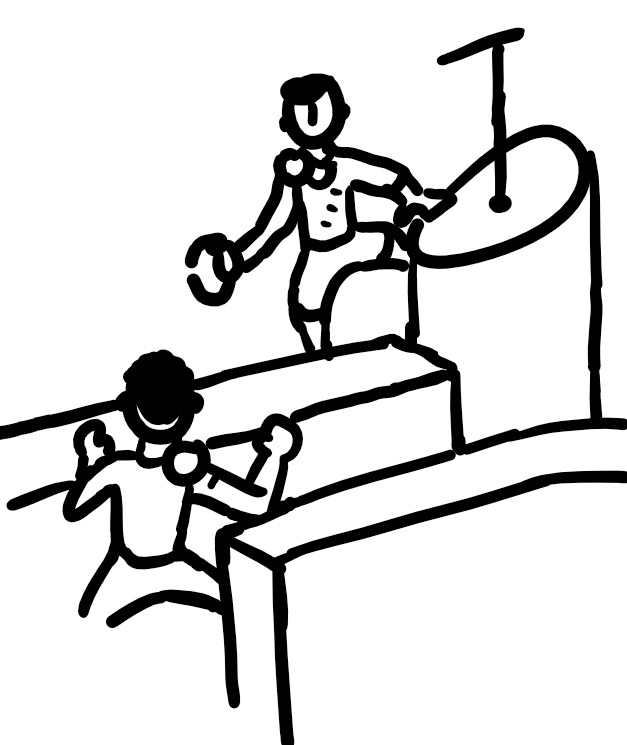
\includegraphics[width=\columnwidth]{sisik.png}}
\entry{taspa u-tesa}{\sense[idiom] kingdom}
\entry[pos=noun]{tesa}{\sense shoreline, bank; where a moving body of water meets the land \sense[of people] hair line}
\entry[pos=noun,sound=/teukkánŏs/,etym=Farlands \fz{tiēkᵛkános}]{teukkanas}{\sense[(\rz{Véajan}) ntr.] missionary, pastor; travelling evangelist who starts local chapters of faith centers \sense[humorous] tourist, vacationer}

% ===== U =====
\addsec{U}

% ===== V =====
\addsec{V}
\entry[pos=noun,sound=/véă(n)jŏ/,etym=Farlands \fz{vḗzșā}]{véaja}{\sense[ntr.] karma; recompense for virtuous behavior \sense[ntr. pl. prox.] a minority religion characterized by proselytization and belief in an afterlife \sense[\rzc\bf sesam véaja] preach, orate: \rz{rappahan sesamzí véaja ez-ǫkas esyi tę-laczin} “the minister preached of an eternal reward for the faithful”}

% ===== Y =====
\addsec{Y}
\entry[pos=noun,sound=/yerrŏ(n)gín/,etym={OL₂ \pz{yer-vŏngín}, Farlands \fz{iēlunzșín}}]{yerragín}{\sense[(\rz{Véajan}) ntr.] a prayer ceremony for greeting a visitor as a show of hospitality \sense[\rzc\bf tahąt osc-yerragín] lead the prayer ceremony \sense[idiom \rzc\bf yiat yerragín] show off, grandstand, put on airs: \rz{egi cuvarąn yiací yerragín tę-ahka im-nassoin} “the king knew the jester was only showing off”}

% ===== Z =====
\addsec{Z}

\end{multicols}

\backmatter
\pagelayout{wide}

\end{document}
